\section{Верификация модели метода сухого электронно-лучевого травления резиста} \label{sec:verification}

Для верификации разработанной модели методом СЭЛТР были получены периодические структуры в слое ПММА на кремниевой подложке. Как и в более ранних работах, использовался резист PMMA 950K A2 от компании ``Allresist'', начальная толщина слоя ПММА составляла 500 нм. Экспонирование производилось в рабочей камере растрового электронного микроскопа CAMSCAN S-4, который был модифицирован для возможности нагрева образца. Давление в камере микроскопа находилось на уровне 10$^{\text{-5}}$ мбар, энергия электронного пучка составляла 20 кэВ, диаметр пучка -- около 600 нм.

Экспонирование резиста производилось ``в кадр'' с размером кадра 2.4$\times$1.9~мм$^\text{2}$, число линий в кадре равнялось 625. Ток экспонирования $I$ находился в диапазоне 4.56--5.62 нА, время экспонирования $t_\mathrm{exp}$ варьировалось от 100 до 200 с, таким образом, доза экспонирования на единицу длины линии $D_\mathrm{l}$ находилась в диапазоне 3.00--7.38 нКл/см. Температура образцов при экспонировании $T$ варьировалась от 130 до 150~$^\circ$C, скорость охлаждения подложки после экспонирования составляла около 0.2~$^\circ$C/с (экспериментальная кривая охлаждения приведена на рисунке~\ref{fig:exp_cooling}). При снижении температуры образца примерно до 50~$^\circ$C он извлекался из камеры микроскопа. Профили линий были получены методом атомно-силовой микроскопии с использованием микроскопа Nanopics 2100.

\begin{figure}[h!]
	\begin{center}
		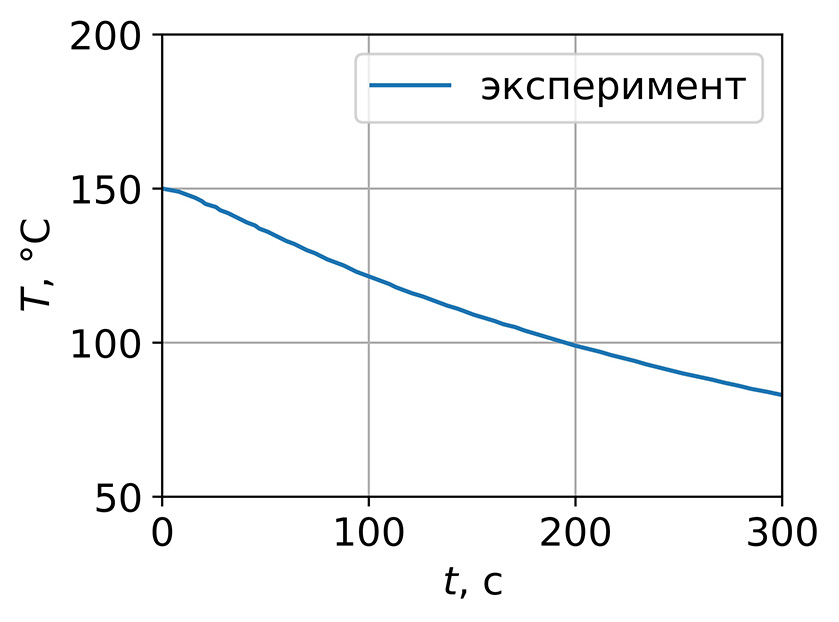
\includegraphics[width=0.5\linewidth]{DEBER_verification/cooling_FINAL_200} \\
	\end{center}
	\vspace{-1em}
	\caption{Экспериментальная зависимость температуры подложки образца от времени при охлаждении после экспонирования.}
	\label{fig:exp_cooling}
	\vspace{1em}
\end{figure}

Полученные в эксперименте профили были промоделированы с использованием модели, описанной выше (рисунок~\ref{fig:DEBER_3D_sim}).
\begin{figure}[h!]
	\begin{center}
		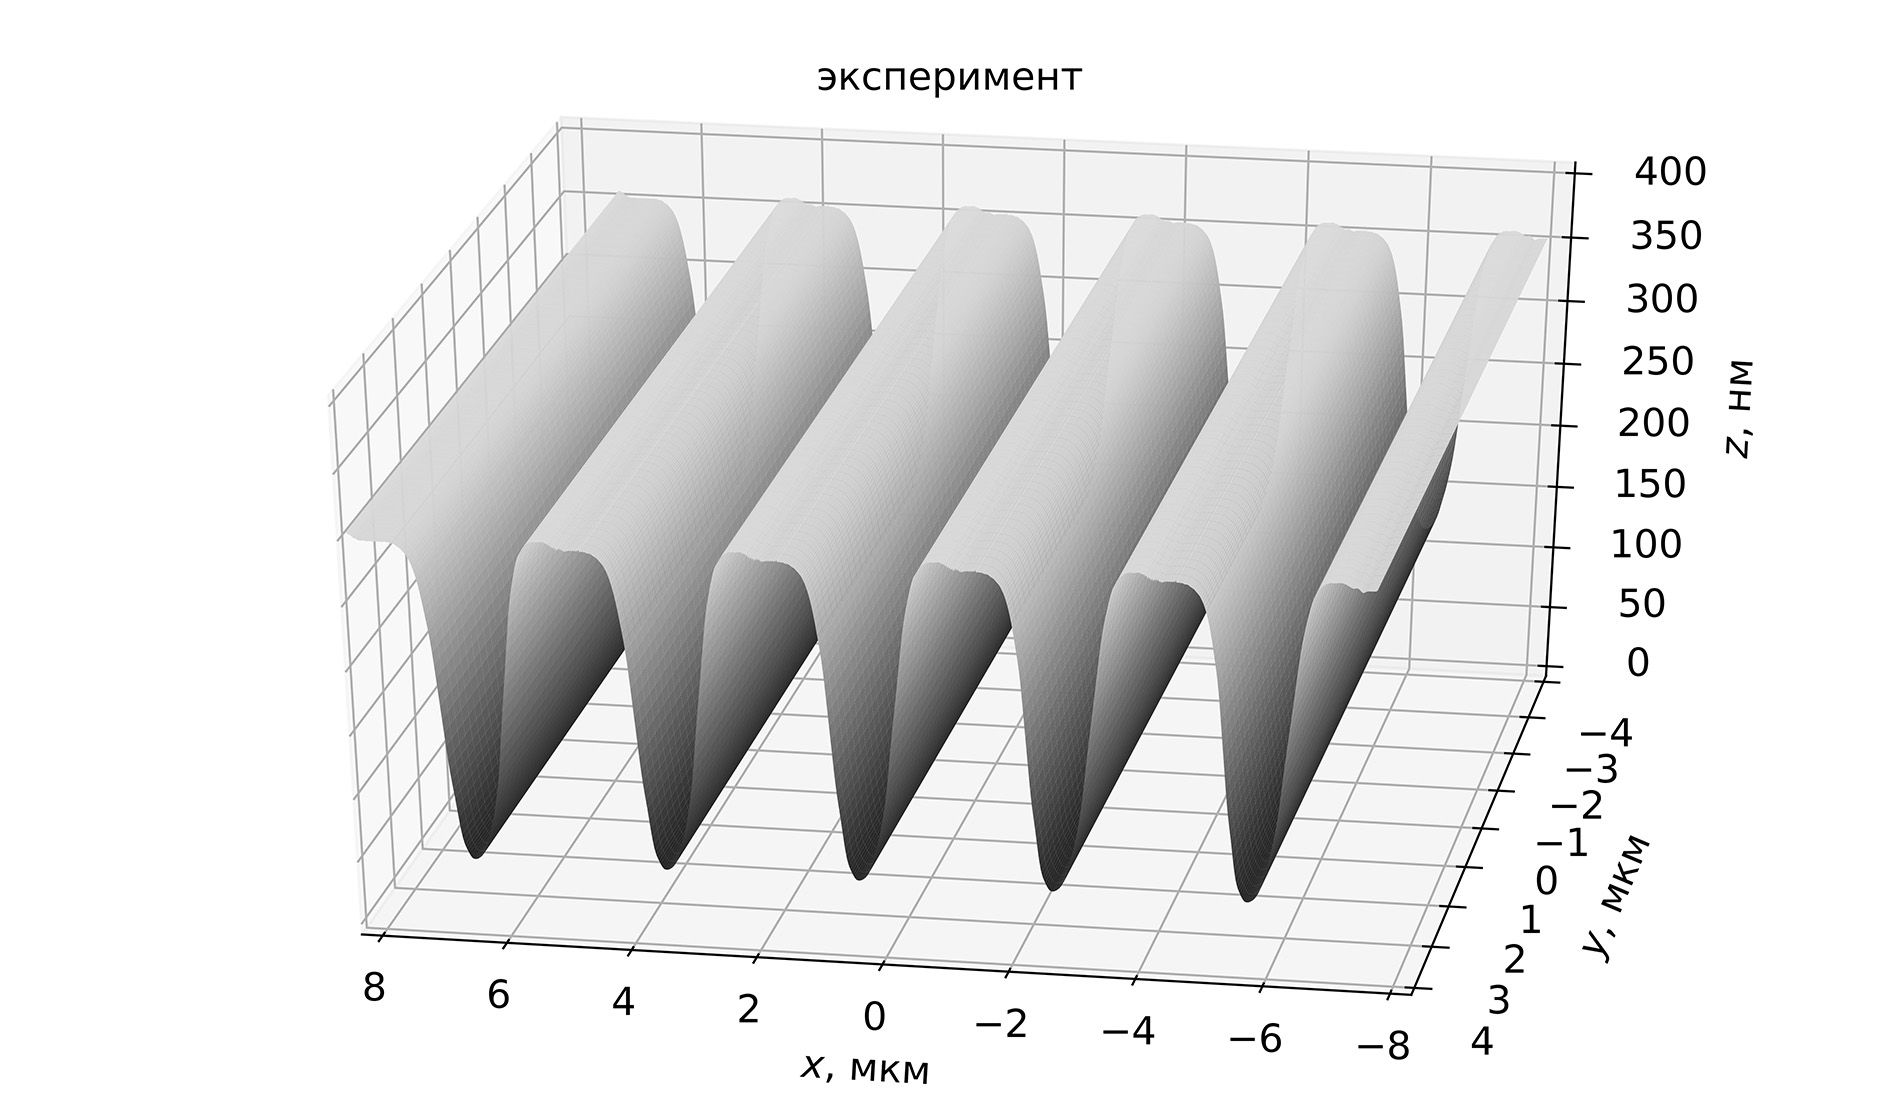
\includegraphics[width=\linewidth]{DEBER_verification/366_EXP_2_50_title_200} \\
		\vspace{-10.7em} \text{\hspace{-25em} a)} \vspace{9.7em} \\
		\vspace{-1em}
		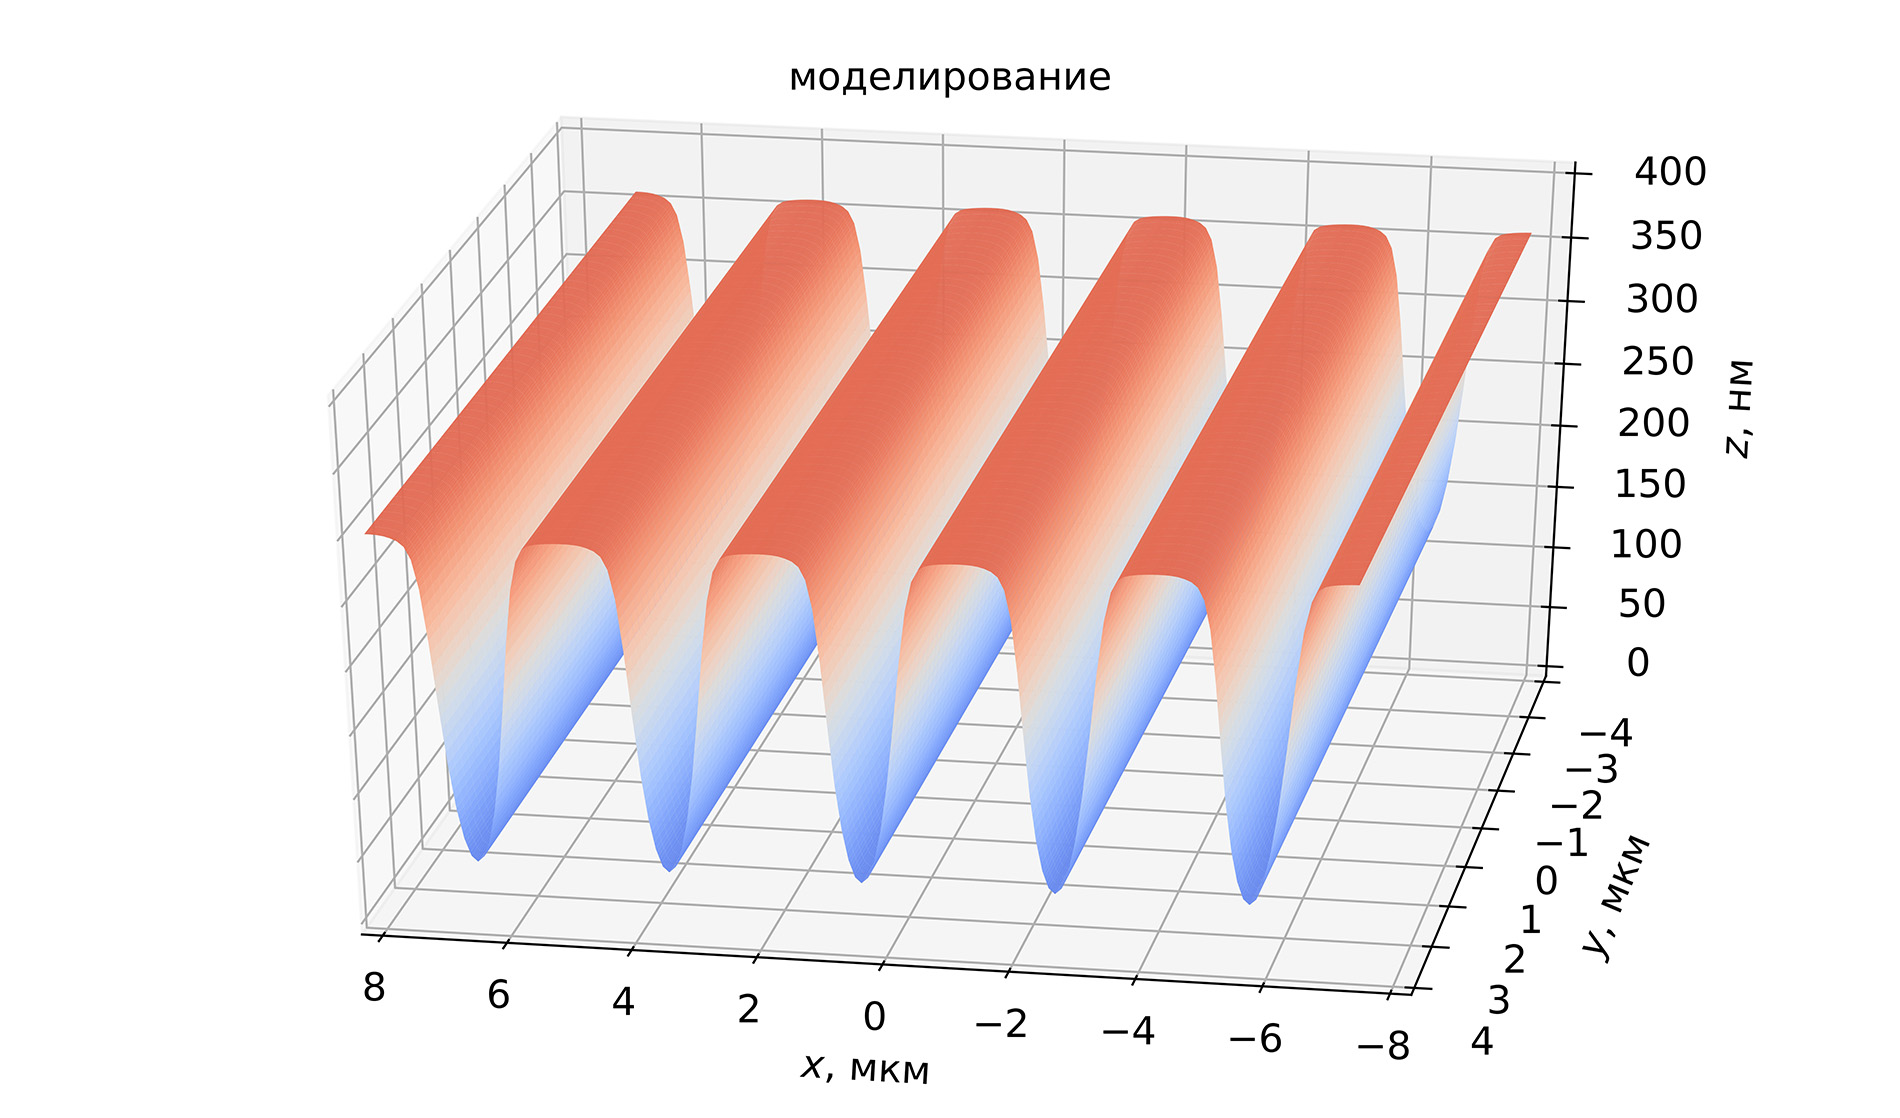
\includegraphics[width=\linewidth]{DEBER_verification/366_SIM_50_2_title_200} \\
		\vspace{-10.7em} \text{\hspace{-25em} б)} \vspace{10.7em} \\
	\end{center}
	\vspace{-2em}
	\caption{Трехмерное изображение поверхности структуры, полученной методом СЭЛТР при $T$ = 150~$^\circ$C, $t_\mathrm{exp}$ = 100 c, $I$ = 4.56 нА (a)) и поверхности, полученной при моделировании (б)).}
	\label{fig:DEBER_3D_sim}
\end{figure}
Для снижения требуемого машинного времени моделирование проводилось для участка одной линии длиной 100 нм, и влияние соседних линий учитывалось за счет использования периодических граничных условий. Число разрывов молекул ПММА, локальная среднечисловая молекулярная масса ПММА и объем микрополостей вычислялись для ячеек размерами 100$\times$100$\times$5 нм$\ppp$ (по осям $x$, $y$ и $z$, соответственно).

Для учета стохастической природы алгоритма моделирования для каждого из экспериментальных профилей проводилось 100 независимых моделирований. Далее на основе профилей, полученных в отдельных моделированиях, рассчитывался усредненный промоделированный профиль. Здесь и далее термин ``промоделированный профиль'' будет обозначать профиль, полученный именно таким образом. Сравнение экспериментальных и промоделированных профилей приведено на рисунке~\ref{fig:DEBER_4_profiles}. Высокая степень воспроизведения экспериментальных профилей указывает на достоверность разработанной модели метода СЭЛТР. Было также установлено, что при описанных выше параметрах экспонирования средняя длина кинетической цепи при деполимеризации ПММА остается постоянной на протяжении первых 100 с процесса, и ее значения составляют 100 и 150 для температур 130 и 150~$^\circ$C соответственно. При дальнейшем экспонировании средняя длина кинетической цепи снижается, и на временном промежутке 100-200 с ее значения составляют 30 и 70 для температур 130 и 150~$^\circ$C соответственно.

\begin{figure}[h!]
	\begin{minipage}{0.48\textwidth}
		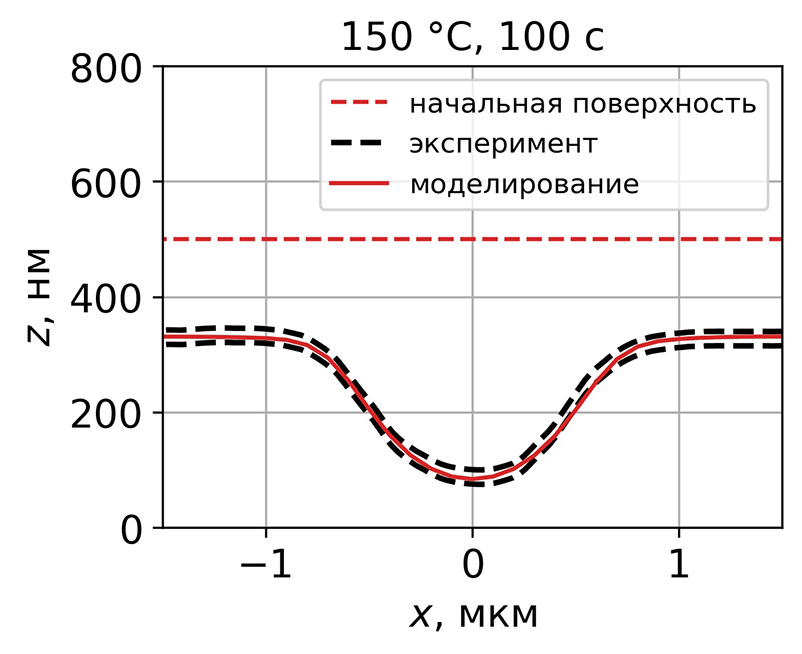
\includegraphics[width=\linewidth]{DEBER_verification/150C_100s_14_FINAL_200} \\
		\vspace{-13em} \\ \text{\hspace{0em} a}) \\ \vspace{13em}
	\end{minipage}
	\begin{minipage}{0.48\textwidth}
		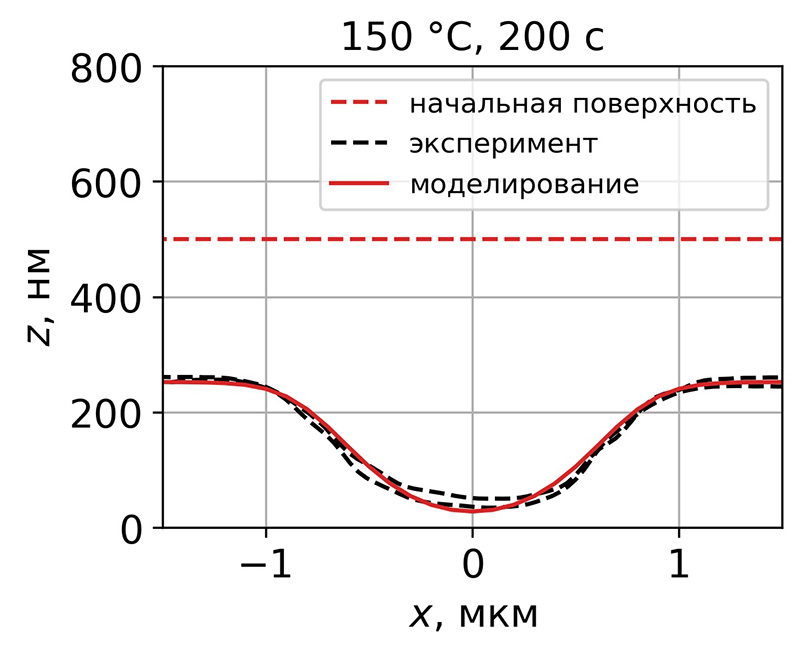
\includegraphics[width=\linewidth]{DEBER_verification/150C_200s_14_FINAL_200} \\
		\vspace{-13em} \\ \text{\hspace{-0.1em} б}) \\ \vspace{13em}
	\end{minipage}

	\vspace{-3em}

	\begin{minipage}{0.48\textwidth}
		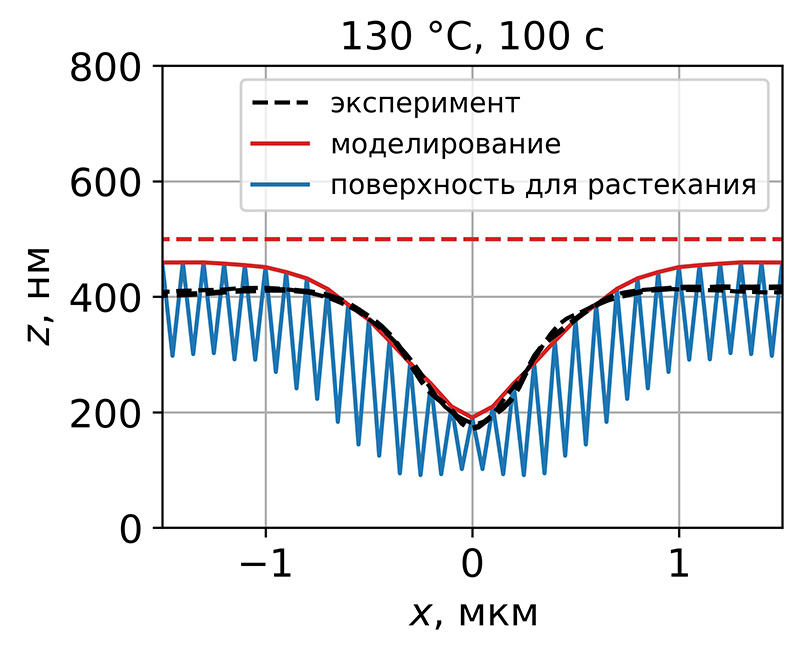
\includegraphics[width=\linewidth]{DEBER_verification/130C_100s_14_FINAL_200} \\
		\vspace{-13em} \\ \text{\hspace{0em} в}) \\ \vspace{13em}
	\end{minipage}
	\begin{minipage}{0.48\textwidth}
		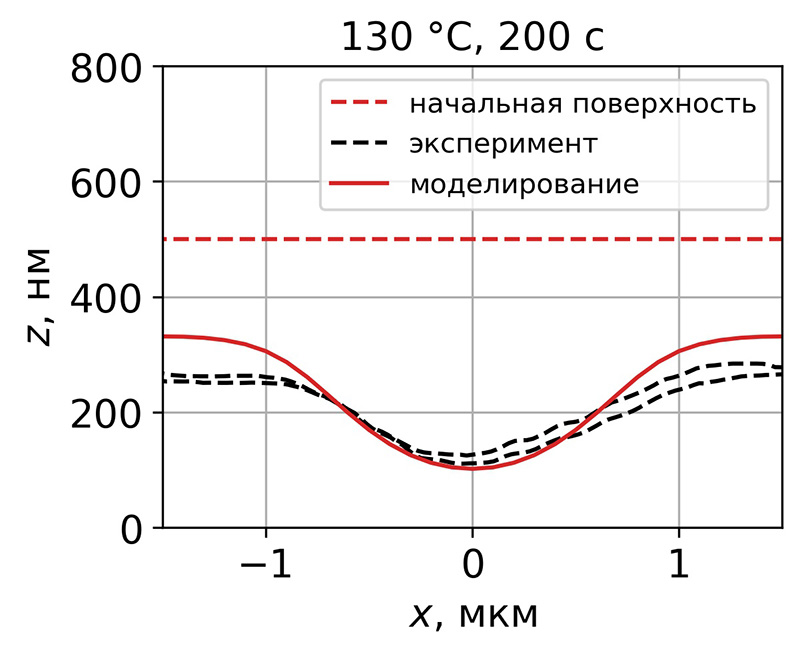
\includegraphics[width=\linewidth]{DEBER_verification/130C_200s_14_FINAL_200} \\
		\vspace{-13em} \\ \text{\hspace{-0.1em} г}) \\ \vspace{13em}
	\end{minipage}
	\vspace{-3em}
	\caption{Верификация разработанной модели процесс СЭЛТР -- сравнение экспериментальных профилей, полученных при экспонировании \linebreak ``в кадр'', с промоделированными профилями для следующих условий экспонирования: a) $T$ = 150~$^\circ$C, $t_\mathrm{exp}$ = 100 c, $D_\mathrm{l}$ = 3.00 нКл/см; б) $T$ = 150~$^\circ$C, $t_\mathrm{exp}$ = 200 c, $D_\mathrm{l}$ = 6.73 нКл/см; в) $T$ = 130~$^\circ$C, $t_\mathrm{exp}$ = 100 c, $D_l$ = 3.12 нКл/см; \linebreak г) $T$ = 130~$^\circ$C, $t_\mathrm{exp}$ = 200 c, $D_\mathrm{l}$ = 7.38 нКл/см. Во всех случаях начальная энергия электронного пучка составляет 20 кэВ, диаметр пучка -- около 600~нм, охлаждение описывается кривой, приведенной на рисунке~\ref{fig:exp_cooling}. Черная пунктирная линия обозначает профили, полученные в эксперименте, красная пунктирная линия -- начальное положение поверхности ПММА, синяя линия -- пилообразную поверхность, использовавшуюся для моделирования растекания слоя ПММА со внутренними микрополостями.}
	\label{fig:DEBER_4_profiles}
	\vspace{1em}
\end{figure}

На рисунке~\ref{fig:DEBER_sigmas} приведены зависимости от $x$-координаты для среднеквадратичного отклонения точек промоделированных профилей, полученные на основе 100 отдельно промоделированных профилей для каждого набора параметров экспонирования. Из рисунка видно, что для профилей, полученных при полном заполнении микрополостей внутри слоя ПММА на момент остывания образца, среднеквадратичное отклонение точек профиля составляет от 0.5 до 3 нм со средним значением около 2 нм. Однако, при наличии микрополостей внутри слоя ПММА на момент остывания (образец, приведенный на рисунке~\ref{fig:DEBER_4_profiles}~в)) среднеквадратичное отклонение точек профиля в центре линии превышает 10~нм.

\begin{figure}[t]
	\begin{center}
		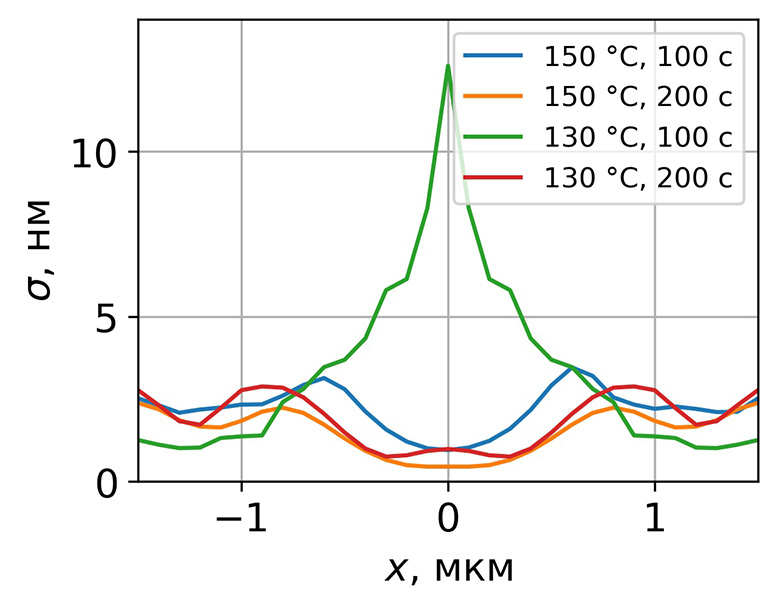
\includegraphics[width=0.5\linewidth]{DEBER_verification/DEBER_sigmas_FINAL_200}
	\end{center}
	\vspace{-1em}
	\caption{Зависимости от $x$-координаты для среднеквадратичного отклонения точек промоделированных профилей, полученные для каждого набора параметров экспонирования.}
	\label{fig:DEBER_sigmas}
	\vspace{1em}
\end{figure}
